\documentclass{beamer}
\usetheme{CambridgeUS}
\usepackage[latin1]{inputenc}
\usepackage[danish]{babel}

\title{Midtvejspr�sentation}
\subtitle{3. sem. projekt}
\author[LBL, RH, KSO, FH, AAB, KLS]
	{Leon B. Larsen\and
	Rudi Hansen\and
	Kent S. Olsen\and
	Frederik Hagelsk�r\and
	Alexander A. Brandbyge\and
	Kim L. Schwaner}
\begin{document}

\frame{\titlepage}

\begin{frame}
\frametitle{Oversigt}
\tableofcontents
\end{frame}

%%%%%%%%%%%%%%%%%%%%%%%%%%%%%%%%%%%%%
\section{Gruppens krav og �nsker}
\begin{frame}
\frametitle{Gruppens krav og �nsker}
\pause
\begin{itemize}[<+->]
	\item Multi-platform (win/osx/linux)
	\item G�re kommunikation s� fejlsikker og hurtig som der er tid- og mulighed for
	\item Generisk bibliotek som er uafh�ngigt af ovenp�-liggende applikation
	\item Mulighed for multi-point kommunikation
\end{itemize}
\end{frame}


%%%%%%%%%%%%%%%%%%%%%%%%%%%%%%%%%%%%%
\section{Team roller}
\begin{frame}
\frametitle{Team roller}
\pause
\begin{itemize}[<+->]
	\item Identificere kompetencer ud fra Belbins team rolle model
	\item .. og v�lge det modsatte
\end{itemize}
\begin{figure}
	\centering
	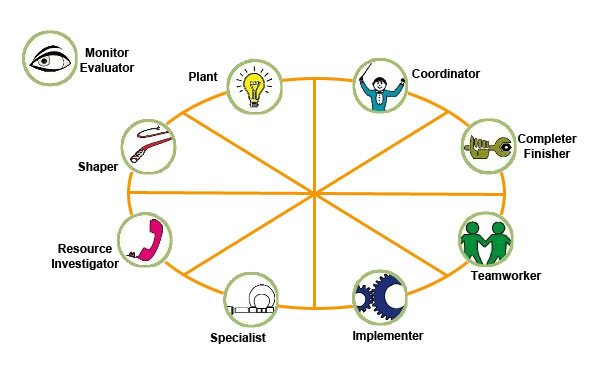
\includegraphics[scale=0.38]{graphics/belbin.jpg}
	\label{fig:belbin}
\end{figure}
\end{frame}


%%%%%%%%%%%%%%%%%%%%%%%%%%%%%%%%%%%%%
\section{Udviklingsv�rkst�jer}
\begin{frame}
\frametitle{Udviklingsv�rkst�jer}
\pause
\begin{itemize}[<+->]
	\item Git(+hub)		
		\begin{itemize}[<+->]
			\item Revisionskontrol
			\item ..b�de til rapport og kodefiler
			\item Alting foreg�r umiddelbart lokalt $\implies$ h�j hastighed $+$ uafh�ngighed
		\end{itemize}
	\item \LaTeX
		\begin{itemize}[<+->]
			\item Typesetting-system
			\item ..g�r det let at skabe ensartede dokumenter, selv med mange input
		\end{itemize}
	\item Trello.com
		\begin{itemize}[<+->]
			\item Online organisering / ''opslagstavle''
			\item Alle kan se hvem, der arbejder p� hvilke opgaver
		\end{itemize}
\end{itemize}
\end{frame}
%Git is a distributed revision control system with an emphasis on speed.[4] Git was initially designed and developed by Linus Torvalds for Linux kernel development. Every Git working directory is a full-fledged repository with complete history and full revision tracking capabilities, not dependent on network access or a central server
%%%%%%%%%%%%%%%%%%%%%%%%%%%%%%%%%%%%%
\section{Lydbibliotek}

\subsection{Krav spec.}
\begin{frame}
\frametitle{Lydbibliotek}
\pause
\begin{itemize}[<+->]
	\item Cross-platform
	\item ''Let at bruge'' / veldokumenteret
	\item Adgang til r� sample-data (PCM)
	\item Open source
	\item Variabel sample-rate og opl�sning
\end{itemize}
\end{frame}

\subsection{Portaudio API}
\begin{frame}
\frametitle{Portaudio API}
\pause
\begin{figure}
	\centering
	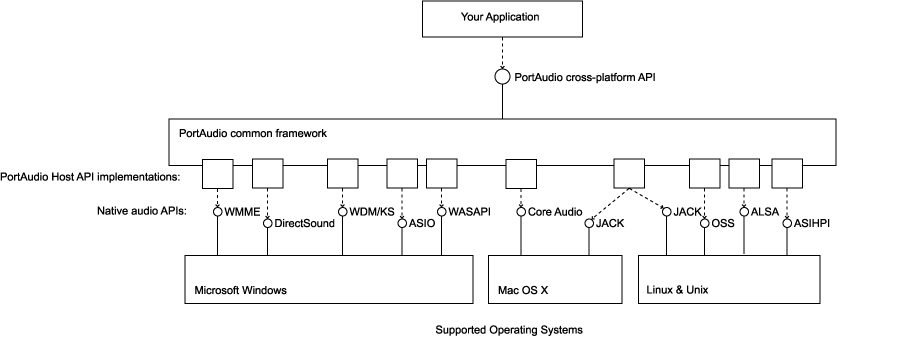
\includegraphics[scale=0.4,trim=0 0 0 20]{graphics/portaudio-external-architecture-diagram.png} %l b r t
	\label{fig:portaudio-external-architecture-diagram}
\end{figure}
\end{frame}

%%%%%%%%%%%%%%%%%%%%%%%%%%%%%%%%%%%%%
\section{Lag-opdelt netv�rk}

\begin{frame}
\frametitle{Lag-opdelt netv�rk}
\pause
\begin{itemize}[<+->]
	\item Naturligt at tale om lag (OSI) i det vi arbejder med netv�rk
	\item Giver en opdeling af arbejdsopgaver og rapport
	\item Vi �nsker en ''black-box'' mellem applikation og mikrofon/h�jtaler p� hver node p� netv�rket
\end{itemize}
\end{frame}

\subsection{''Vores'' lag}
\begin{frame}
\frametitle{''Vores'' lag}
\pause
\begin{figure}
	\centering
		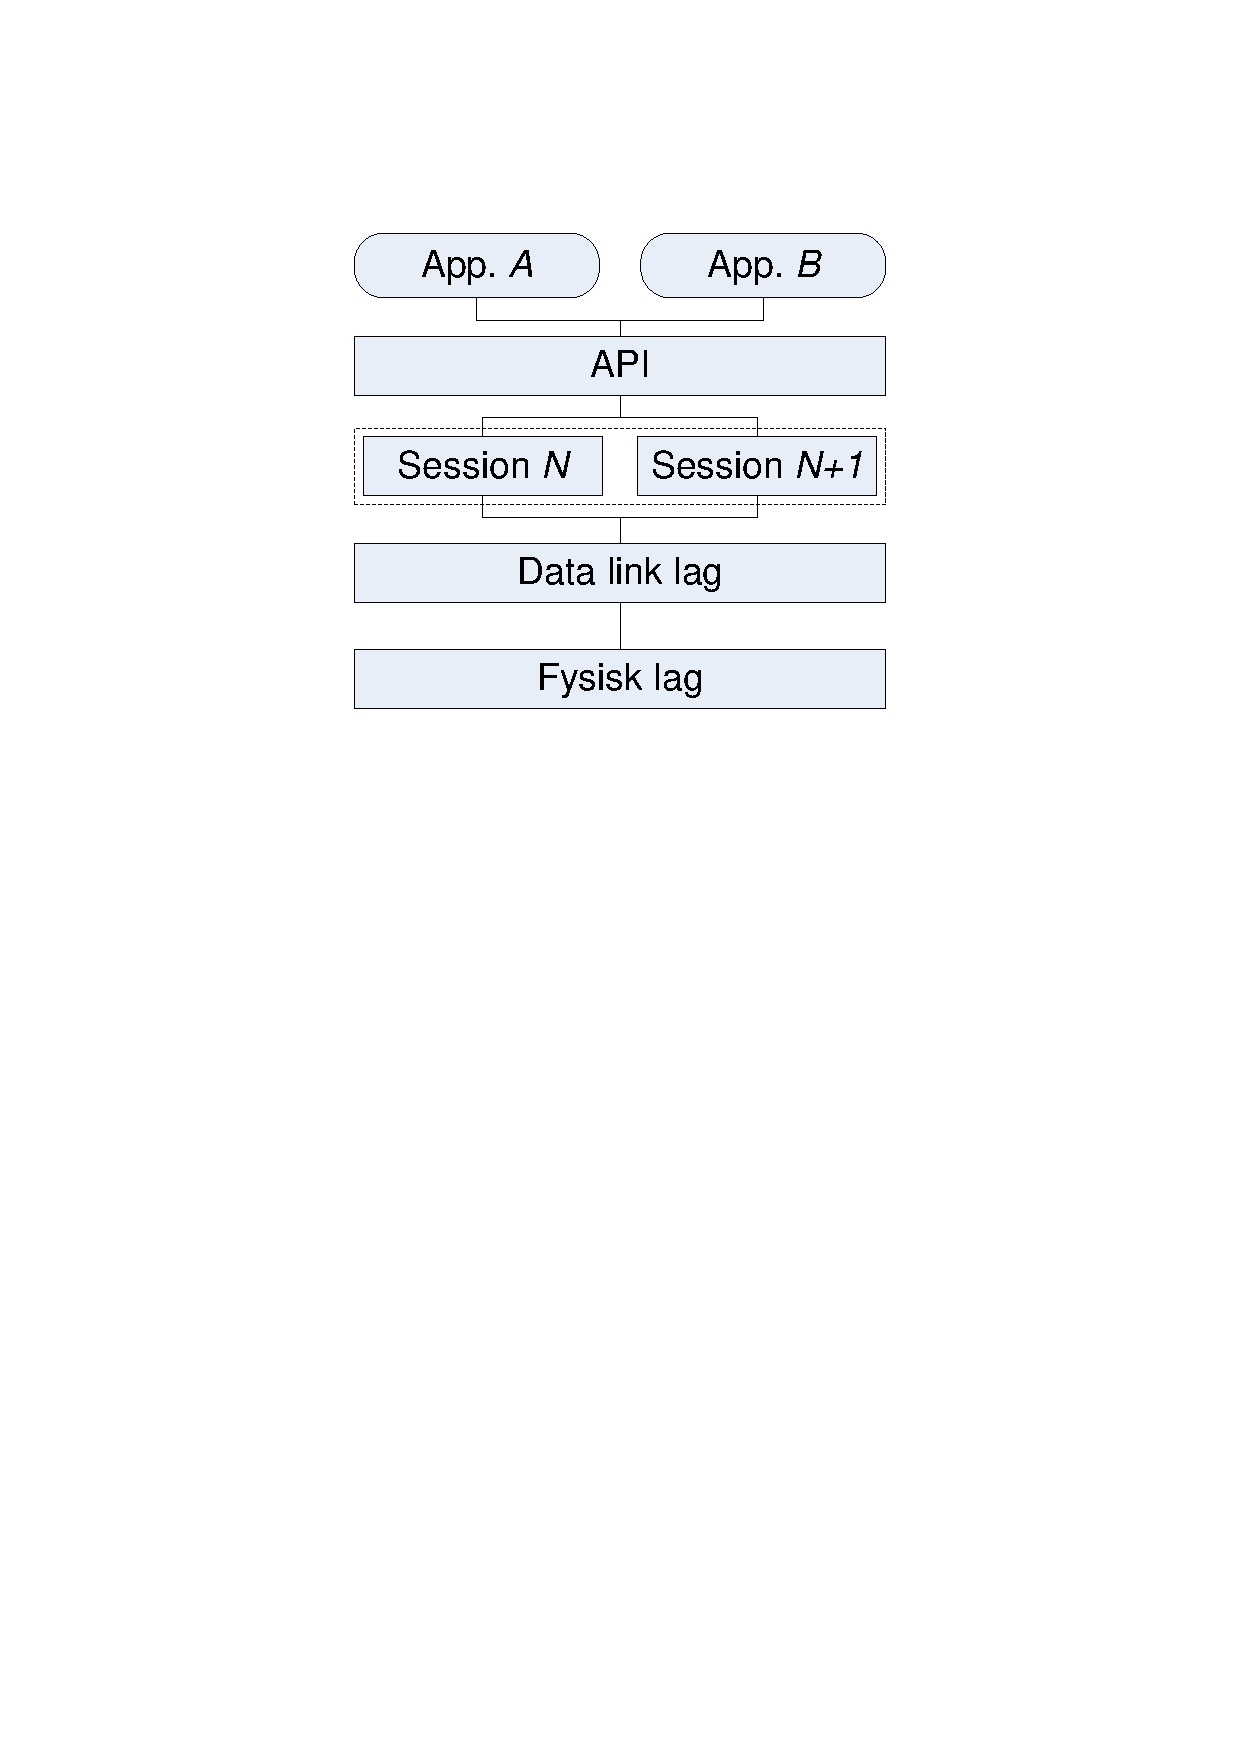
\includegraphics[trim=100 520 100 120,scale=0.6]{graphics/layers.pdf} %l b r t
	\label{fig:layers}
\end{figure}
\end{frame}

%%%%%%%%%%%%%%%%%%%%%%%%%%%%%%%%%%%%%
\section{To-do}

\begin{frame}
\frametitle{To-do}
\pause
\begin{itemize}[<+->]
	\item Pr�cist definere snitflader mellem hvert af vores lag
	\item Udvikle og teste hvert lag for sig
	\item Beslutte hvor stor fejl-kontrol der er brug for (test)
	\item Optimering
	\item Skrive test-applikation
\end{itemize}
\end{frame}

\end{document}